\paragraph{QuizziPedia::Front-End::ModelViews::QuestionnaireQuestionsManagementModelView}
					
					\label{QuizziPedia::Front-End::ModelViews::QuestionnaireQuestionsManagementModelView}
					
					\begin{figure}[ht]
						\centering
						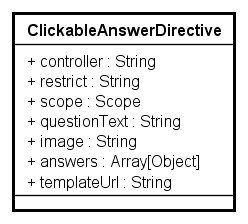
\includegraphics[scale=0.5,keepaspectratio]{UML/Classi/Front-End/QuizziPedia_Front-end_Templates_ClickableAnswerTemplate.png}
						\caption{QuizziPedia::Front-End::ModelViews::QuestionnaireQuestionsManagementModelView}
					\end{figure} \FloatBarrier
					
					\begin{itemize}
						\item \textbf{Descrizione}: classe di tipo modelview la cui istanziazione è contenuta all'interno della variabile di ambiente \$scope di \textit{Angular.js\ped{G}}. All'interno di essa sono presenti le variabili e i metodi necessari per il \textit{Two-Way Data-Binding\ped{G}} tra la view \texttt{QuestionnaireQuestionsManagementView} e il controller \texttt{QuestionnaireQuestionsManagementController};
						\item \textbf{Utilizzo}: viene utilizzata per effettuare il \textit{Two-Way Data-Binding\ped{G}} tra la view \texttt{QuestionnaireQuestionsManagementView} e il controller \texttt{QuestionnaireQuestionsManagementController} rendendo disponibili variabili e metodi;
						\item \textbf{Relazioni con altre classi}: 
						\begin{itemize}
							\item \textit{IN} \texttt{CreateQuestionnaireView}: view per la creazione del questionario; 
							\item \textit{IN} \texttt{QuestionnaireQuestionsManagementController}: questa classe permette di gestire il recupero delle parole chiave di un questionario;
						\end{itemize}
						\item \textbf{Attributi}: 
						\begin{itemize}
							\item ;
						\end{itemize}
						\item \textbf{Metodi}: 
						\begin{itemize}
							\item ;
						\end{itemize}
					\end{itemize}
					
						
							